\section{Methodology}

The system's observation mode can take two states: ``monitoring mode'' or ``alert mode''. 
We tested a variety of detectors to ingest pressure time series and determine the probability of a dust devil event. 
We rely on past data to develop and measure engineering performance of the detectors as well as conduct a science evaluation of the overall system.

Detectors ingest time-series data to generate the confidence that the rover is encountering a vortex.
Given these confidence values, the detectors trigger a transition to the alert mode when a configurable threshold is met. 
On a real mission, the spacecraft would initiate higher power and data volume instruments to capture these vortex events.
As described in Section \ref{subsec:evaluation}, we quantify the ability of each detector to trigger during the 60 second window leading up to the \textit{start} of an eyewall encounter. 
That any useful detector must identify the early signs of a vortex to enable the spacecraft to react and capture the main scientific value of the event.
As soon as the spacecraft enters alert mode, it starts 180-second cooldown timer (though the length is configurable). 
Once the timer runs out, the spacecraft returns to monitoring mode. 
The timer is restarted if the confidence threshold is met again during the alert mode.

\begin{figure}
    \centering
    \includegraphics[width=0.45\textwidth]{example-image.pdf}
    \caption{The observation mode fluctuates between two states in response to the in situ environment. In ``Monitoring Mode,'' the spacecraft is relatively quiescent. It collects data from low power sensors at a low rate (e.g., only pressure sensor readings at \unit[1]{Hz}). If a dust devil is detected, the system enters an alert mode collecting data with all relevant sensors at high rate (e.g., NavCam images). After a configurable amount of time (e.g., \unit[60]{s}) without another detection, the system will return to monitoring mode.}
    \label{fig:Population_Weighted_Dust_Flux}
\end{figure}

\subsection{Data and Preprocessing}\label{subsection:data}
\textit{Takeaways: origin of data, preprocessing/labels connected connections to Jackson, 2022}

To compile our vortex dataset, we used data from the \acrfull{MEDA} instrument suite aboard the Mars 2020 Perseverance rover. \acrshort{MEDA} collects data using a number of meteorological instruments including a pressure sensor and a radiation and dust sensor. Its data is useful for studying a number of processes related to both short- and long-term events of interest including convective vortices. Along with the \unit[1]{Hertz} pressure sensor data, we also use previously identified vortices from \cite{Jackson2022}. This work applied a detection scheme that detrends the data using a moving average (Boxcar filter), convolves the time-series data a Lorentzian profile to find vortex-like signals, and then finds uses a threshold to find periods in the time series most resembling the Lorentzian template. The authors identified 309 vortex signals in M2020's first 89 sols, which are included in a machine readable table.

Using these known vortices, we compiled \acrshort{ML}-ready data to train and evaluate multiple detection schemes. 
At a high level, this involved combining the raw pressure time series (from \acrshort{PDS}) with timing information from previously known dust devils. 
We used data from \cite{Jackson2022} to add binary columns identifying all points in the time series that were within the \acrfull{FWHM} of a vortex, within the 60-second detection window before the start of the \acrshort{FWHM}, 4$\times$ the \acrfull{FWHM} of a vortex, and the vortex index (from the original vortex annotations data). The \acrshort{FWHM} is a proxy for the high-science-value period thought to be when the rover is within the vortex eyewall. As described at the start of this section, the a successful detection only occurs if the detector initiates an alert before the start of the \acrshort{FWHM} to provide an opportunity for other instruments to turn on or adapt. Thus, we evaluate the detectors ability to trigger during the detection window. The 4$\times$ \acrfull{FWHM} feature captures a wide period of time around the vortices and is useful for training algorithms to detect any signs of a vortex. Finally, we use the vortex index to map all detections and misses back to the vortex metadata compiled in \cite{Jackson2022} to characterize any biases in the detectors. These metadata include measurements like the depth of the pressure excursion, length of the vortex encounter, etc.

\begin{figure}
    \centering
    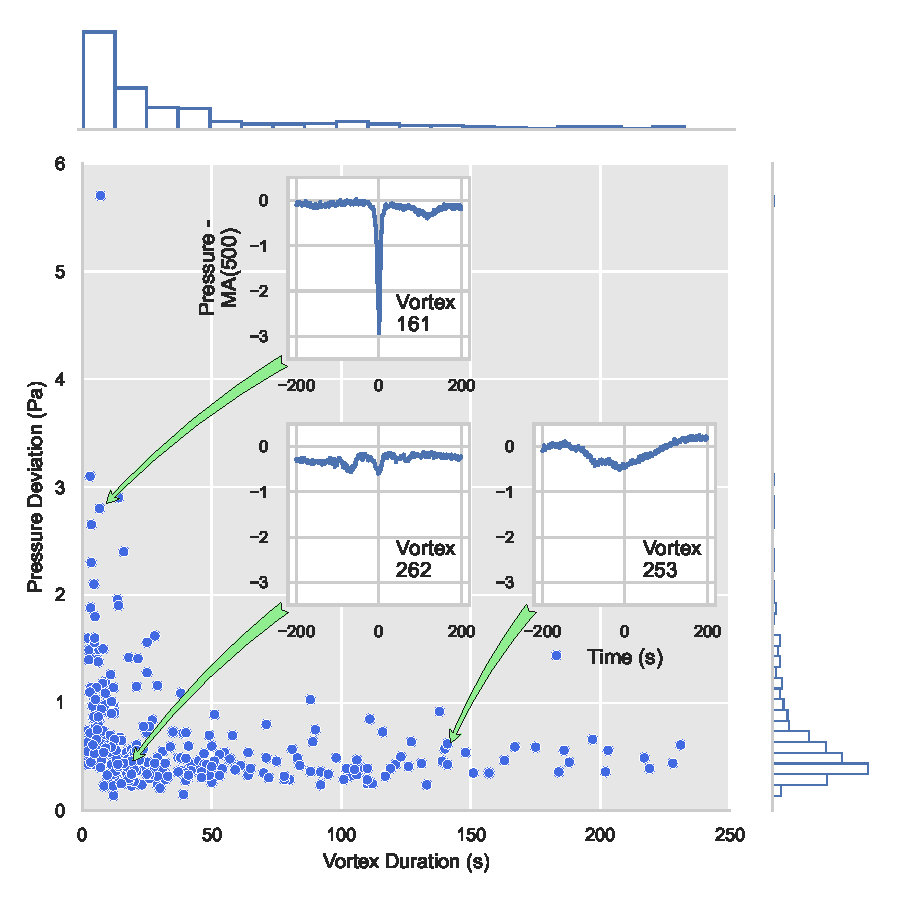
\includegraphics[width=0.8\textwidth]
    {figures/manuscript_vortex_dur_pres_dists_v4.pdf}
    \caption{Distribution of vortex pressure deviations and durations. Most vortices tended to have a small pressure deviation ($<$1Pa) and short duration ($<$50s; lower left). However, there are two exceptions: short duration, high pressure deviations vortices and long lasting, small deviation vortices. The duration and strength of the pressure deviation is an important consideration for any detection algorithm. There is no obvious difference between vortices with or without dust.}
    \label{fig:vortex_dur_pres_dists}
\end{figure}

\subsection{Vortex Detectors}\label{subsection: vortex_detectors}
\textit{Takeaways: Describe the input/output of each detector, the technical details behind 3 detection methods}

We developed and tested three different vortex detectors that ranged in complexity and training data requirements: (1) a simple statistical outlier detector, (2) an adaptive statistical outlier detector and (3) and an \acrshort{ML}-based \acrfull{LSTM} model. 
For each, we used the data described in Section \ref{subsection:data} to conduct a \acrfull{HPO} search to determine the best parameters for each detector. 
For each individual \acrshort{HPO} trial, the first 80\% of the data was used for a 5-fold cross validation with scikit-learn’s time series split tool to obtain a more representative estimate of performance. 
The \acrfull{ROC AUC} metric was used as our target metric because it is more representative of the holistic performance over a range of probability thresholds. 
We leveraged the Ray library to execute the \acrshort{HPO} search in a parallelized manner. 
After cross validation, a final model was trained on the entire training dataset with the best set of parameters and tested on the held out 20\% of the data. 

\subsubsection{Low Complexity: Statistical Outlier Detector}
\begin{figure}
    \centering
    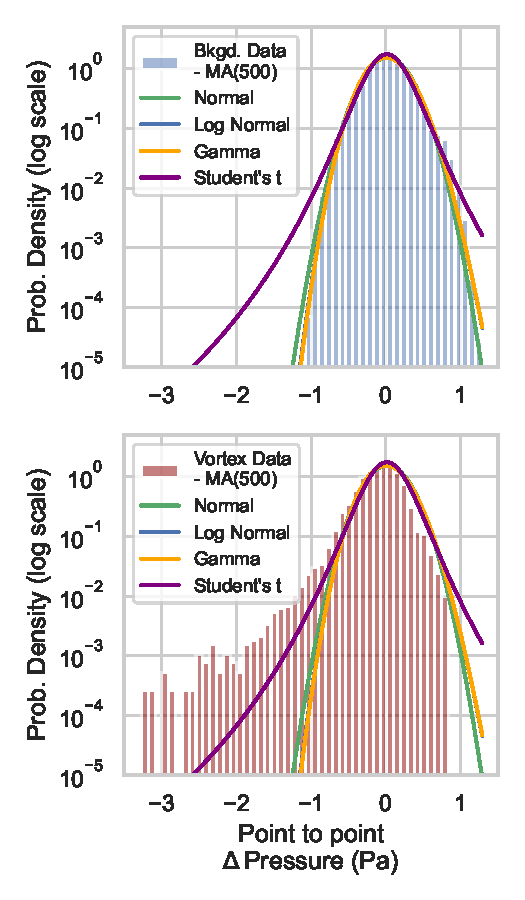
\includegraphics[width=0.45\textwidth]    {figures/manuscript_static_detector_overview_fig_v3.pdf}
    \caption{Statistical distributions fit to background data (top) can be used to detect statistical deviations from backgrounds during vortex events (bottom). (Top) We used normal, log normal, and gamma distributions to fit the detrended background data, but the Student's t distribution was also included to illustrate that many distributions led to poor fits. (Bottom) When comparing distribution fits to vortex data, negative pressure deflections reside in a heavy tail falling outside the background distribution making them useful for detecting vortices. Note the abrupt end on the \textit{positive} tail is due to the moving average filter incorporating vortices' initial negative deflection. See Figure \ref{fig_appendix:vortex_press_diff_without_bkgd_subtraction_dist_fit} in the Appendix for more information.}
    \label{fig:detector1_overview}
\end{figure}

The simple statistical outlier detector uses the simplest conceptual approach to detect vortices. 
It fits a static distribution to the background training data and uses it to identify outliers in the incoming pressure measurements. 
All data points outside 4$\times$\acrshort{FWHM} of a known vortex were extracted and used to fit several distributions (Figure \ref{fig:detector1_overview}). 
Once generating a distribution fit, we can calculate the \acrfull{CDF} up to the incoming data point to estimate the probability of observing a pressure reading at least as extreme as the incoming measurement. 
We then take $1-CDF(x)$ as the probability that the current value belongs to a vortex (such that very small \acrshort{CDF} values translate to high probabilities).
Note that we only use a one-tailed distribution — the left side — since the primary pressure deflection due to a vortex will be negative. 
We used Scipy’s stats module to test a number of distributions including Laplace, Student’s t, non-central Student's t, normal, generalized normal, lognormal, generalized logistic, gamma, double gamma and Levy-stable. 
Only the normal, lognormal, gamma gave reasonable fits, so these were used during the quantitative \acrshort{HPO} step. 
The performance (according to \acrshort{ROC AUC}) was extremely similar for all three. 
The normal distribution showed a very slight edge and is perhaps the most well-known distribution of the three, so we used it when going forward to the event detection evaluation. 

\subsubsection{Medium Complexity: Adaptive Statistical Outlier Detector}

The adaptive statistical outlier detector fits a distribution to a rolling window of input data and then identifies outliers similar to the simple detector. 
As pressure measurements are acquired they are inserted into a short rolling buffer window. 
At each time point, the data is detrended by fitting a linear function to the windowed data and subtracting it off. 
Next, a normal distribution is fit to these residuals. 
For the newest data point, we extrapolate the linear fit to the new point, apply the same detrending, and then calculate the \acrshort{CDF} and vortex probability as before.
Again, we assume a one-tailed distribution since we are focused on detecting negative pressure deviations. 
We tested different window sizes (ranging from 15 to 1000 seconds) and found that the 1000 second window achieved the best performance during cross validation.

\begin{figure}
    \centering
    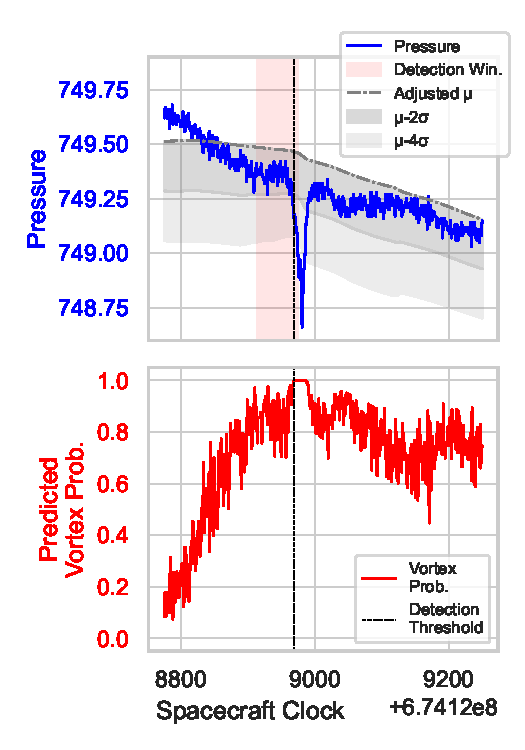
\includegraphics[width=0.45\textwidth]{figures/manuscript_adaptive_detector_overview_fig_v1.pdf}
    \caption{A normal distribution fit to the most recent, mean-subtracted background data (top) can be used to set an adaptive detection threshold for vortex events (bottom).}
    \label{fig:detector2_overview}
\end{figure}

\subsubsection{High Complexity: \acrshort{LSTM} Detector}
The ML-based detector relies on \acrfull{LSTM} model, which is a popular recurrent neural network used for time series analysis. 
The \acrshort{LSTM} architecture includes recurrence — sequentially feeding previous model outputs as future inputs — and builds on this by adding a series of gates to acquire, maintain, and forget information over relatively long time intervals. 
This conveys the capability to learn fairly complex time series data relationships. 
We trained \acrshortpl{LSTM} models with Tensorflow to predict the probability the input time series was within $4\times$\acrshort{FWHM} of a known vortex. 
As vortices are relatively rare, we used class weights to balance the importance of correctly predicting both background and vortex data points. 
Our \acrshort{HPO} experiment ran trails with a range of values for the number of output units (16, 32, 64, or 128), dropout ([0, 0.25]) and recurrent dropout ([0, 0.25]) to reduce overfitting, learning rate ([1e-3 to 1e-2]), used a large batch size of 8192 samples, and a 60 second window of input data. 
After executing the \acrshort{HPO}, we found that a model with \textcolor{red}{(input final details from test results)} performed best.

\subsection{Evaluation}\label{subsec:evaluation}
\textit{Takeaways: Overview of how we quantify the science value }
To evaluate the vortex detectors, we assessed their ability to enable correct transitions between monitoring and alert modes. 
This involved two evaluation steps: (1) assessing the detectors' point probabilities concerning their ability to assign high confidence values to point measurements when experiencing a vortex and (2) assessing the detector to correctly guide the broader system to capture vortex events (e.g., high recall) with the fewest number of false triggers (e.g., high precision). The first step utilized traditional detection theory metrics to help assess detectors within each family. Note that while this was valuable to select the best model architecture during the \acrshort{HPO} process, it is less useful to compare point prediction results across detectors.

The second evaluation assess each detectors ability to correctly translate per-point confidence values into a series of alerts.
On one hand, mission operators and scientists can set a loose filter (using a relatively low threshold) reduce the chances of missing vortices at the cost of increase power and data consumption. 
Such an approach effectively prioritizes science return over onboard resources.
On the other hand, a tight filter (with a relatively high threshold) will conserve power and data at the cost of potentially missing scientifically valuable events. 
This approach effectively prioritizes resource conservation at the cost of missing science events.
Both strategies will likely be valuable depending on the individual mission, its phase, resource usage by other instruments, etc., so we tested both to quantify tradeoffs and inform engineering constraints.

We also explore qualitative considerations like the amount of data required to train each detector and compute complexity.

\subsubsection{Evaluation: Detector Point Estimates}\label{subsubsec:point_evaluation}
\textit{Takeaways: Explain how we quantify performance on individual time points. This was used during HPO}

Therefore, we translated the individual point probabilities into a series of event detections for comparison with the labeled vortices. 
This involved setting a threshold on the point estimates to initiate the start of event detections (corresponding to an alert trigger) and then end the detection when the cooldown timer expires (corresponding to a return to monitoring mode). 
After generating a list of events, we identified true positives as any ground truth vortices in the labeled data where the autonomous event both triggered during the detection window (within 60 seconds of the \acrshort{FWHM} beginning) and overlapped the entire \acrshort{FWHM} period. 
We also misses where the detector didn't capture any portion of the event, near misses as vortices where the trigger was late and occurred during the \acrshort{FWHM}, and possible unlabeled hits where the event window overlaps a  vortex-like pressure deflection that was not annotated in the ground truth dataset.


\subsubsection{Evaluation: Event Detections}
\label{subsec:evaluation_event_detections_methods}
\textit{Takeaways: Explain how we quantify science value of the overall system. Explain value of triggering alert mode *before* FWHM window}

For each detector, we tested both situations by finding thresholds that mapped to a frequency of alerts that collected ~25\% and ~5\% of the original pressure time series data points. 
These results are shown in Table \ref{tab:detection_rates}.


